\documentclass[aps,preprint]{revtex4-2}

\usepackage{amsmath,amsfonts,amssymb,bm}
\usepackage{graphicx}
\usepackage{hyperref}
\usepackage{times}
\usepackage{float}
\usepackage{xr}
\renewcommand{\thefigure}{S\arabic{figure}}
\renewcommand{\thetable}{S\arabic{table}}
% Title and Author Information
\begin{document}

\title{Supplemental Material fo ``Curious Fringe around a Beet Slice''}

\author{Zhengyang Liu}
\affiliation{Department of Biological and Environmental Engineering, Cornell University, Ithaca, NY 14853, USA}
\author{Kunal Kumar}
\author{Yicong Fu}
\author{Ahbradeep Maitra}
\affiliation{Department of Mechanical and Aerospace Engineering, Cornell University, Ithaca, NY 14853, USA}
\author{Justin Chen}
\author{Sunghwan Jung}
\affiliation{Department of Biological and Environmental Engineering, Cornell University, Ithaca, NY 14853, USA}
\date{\today}
\maketitle

\section{Flow measurement}

Flow velocity measurement was done by tracking the motion of tracer particles.
We show that the flow velocity is decaying rapidly over time. 
In the mean time, the fringe pattern can last for a longer time.
This disproved the hyposthesis that the fringe pattern is an example of Reynolds ridge.

\begin{figure}[ht]
    \centering
    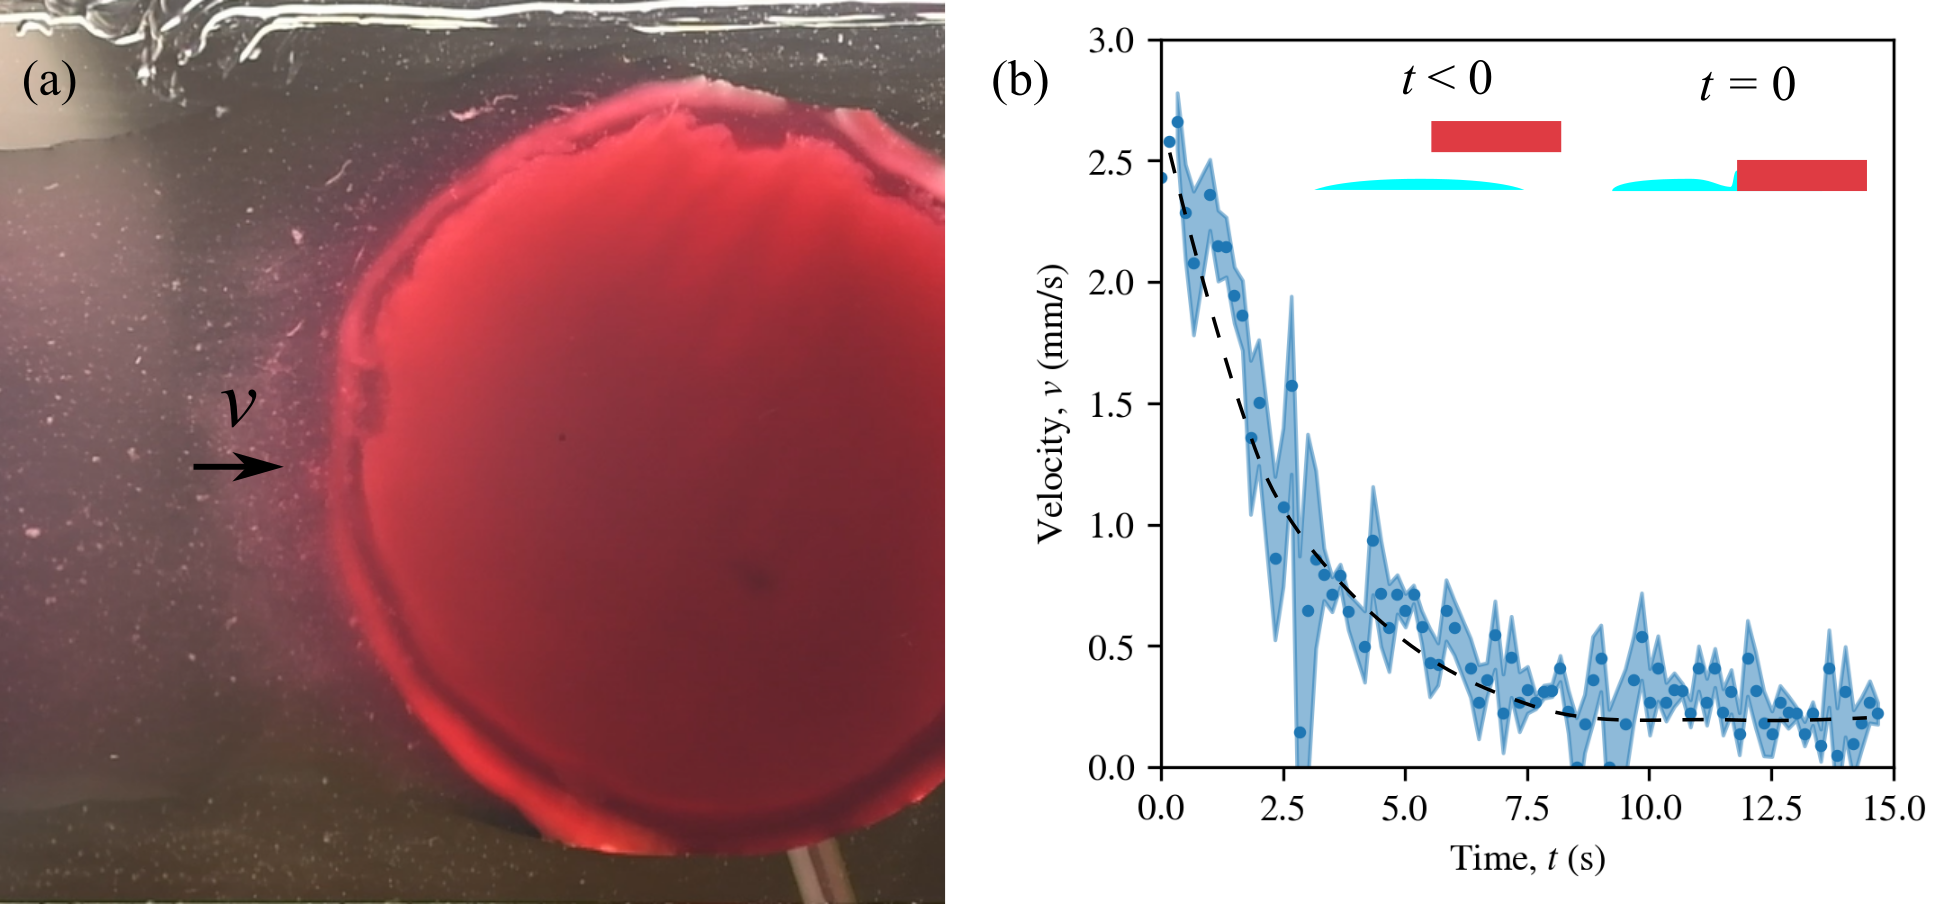
\includegraphics[width=\linewidth]{Figures/beet_flow_measurement.png}
    \caption{
    (a) An image taking by the DSLR camera. The black arrow indicates the location where flow speed is measured.
    (b) Flow speed as a function of time. The insets illustrate a conceptual picture of the dimple formation process.
    }
    \label{fig:flow-measurement}
\end{figure}

\newpage

\section{Extrapolation of surface profiles}

Very close to the vertical wall, the displacement sensor was not able to detect the surface height due to the large slope.
The close-to-wall part of the surface profile was constructed by extrapolation.
The gray curve is the raw data from the displacement sensor. 
The blue part of the curve is used for the extrapolation fitting. The red curve is the extrapolated surface profile. 
The high plateau on the right end of the plot is the top surface of the beet slice, which can be reliably detected by the displacement sensor. 
Our extrapolation therefore only fill in the missing part between the ``tip'' and the beet wall. 
The extrapolation is done by fitting the data with a 3rd order polynomial function.

\begin{figure}[ht]
    \centering
    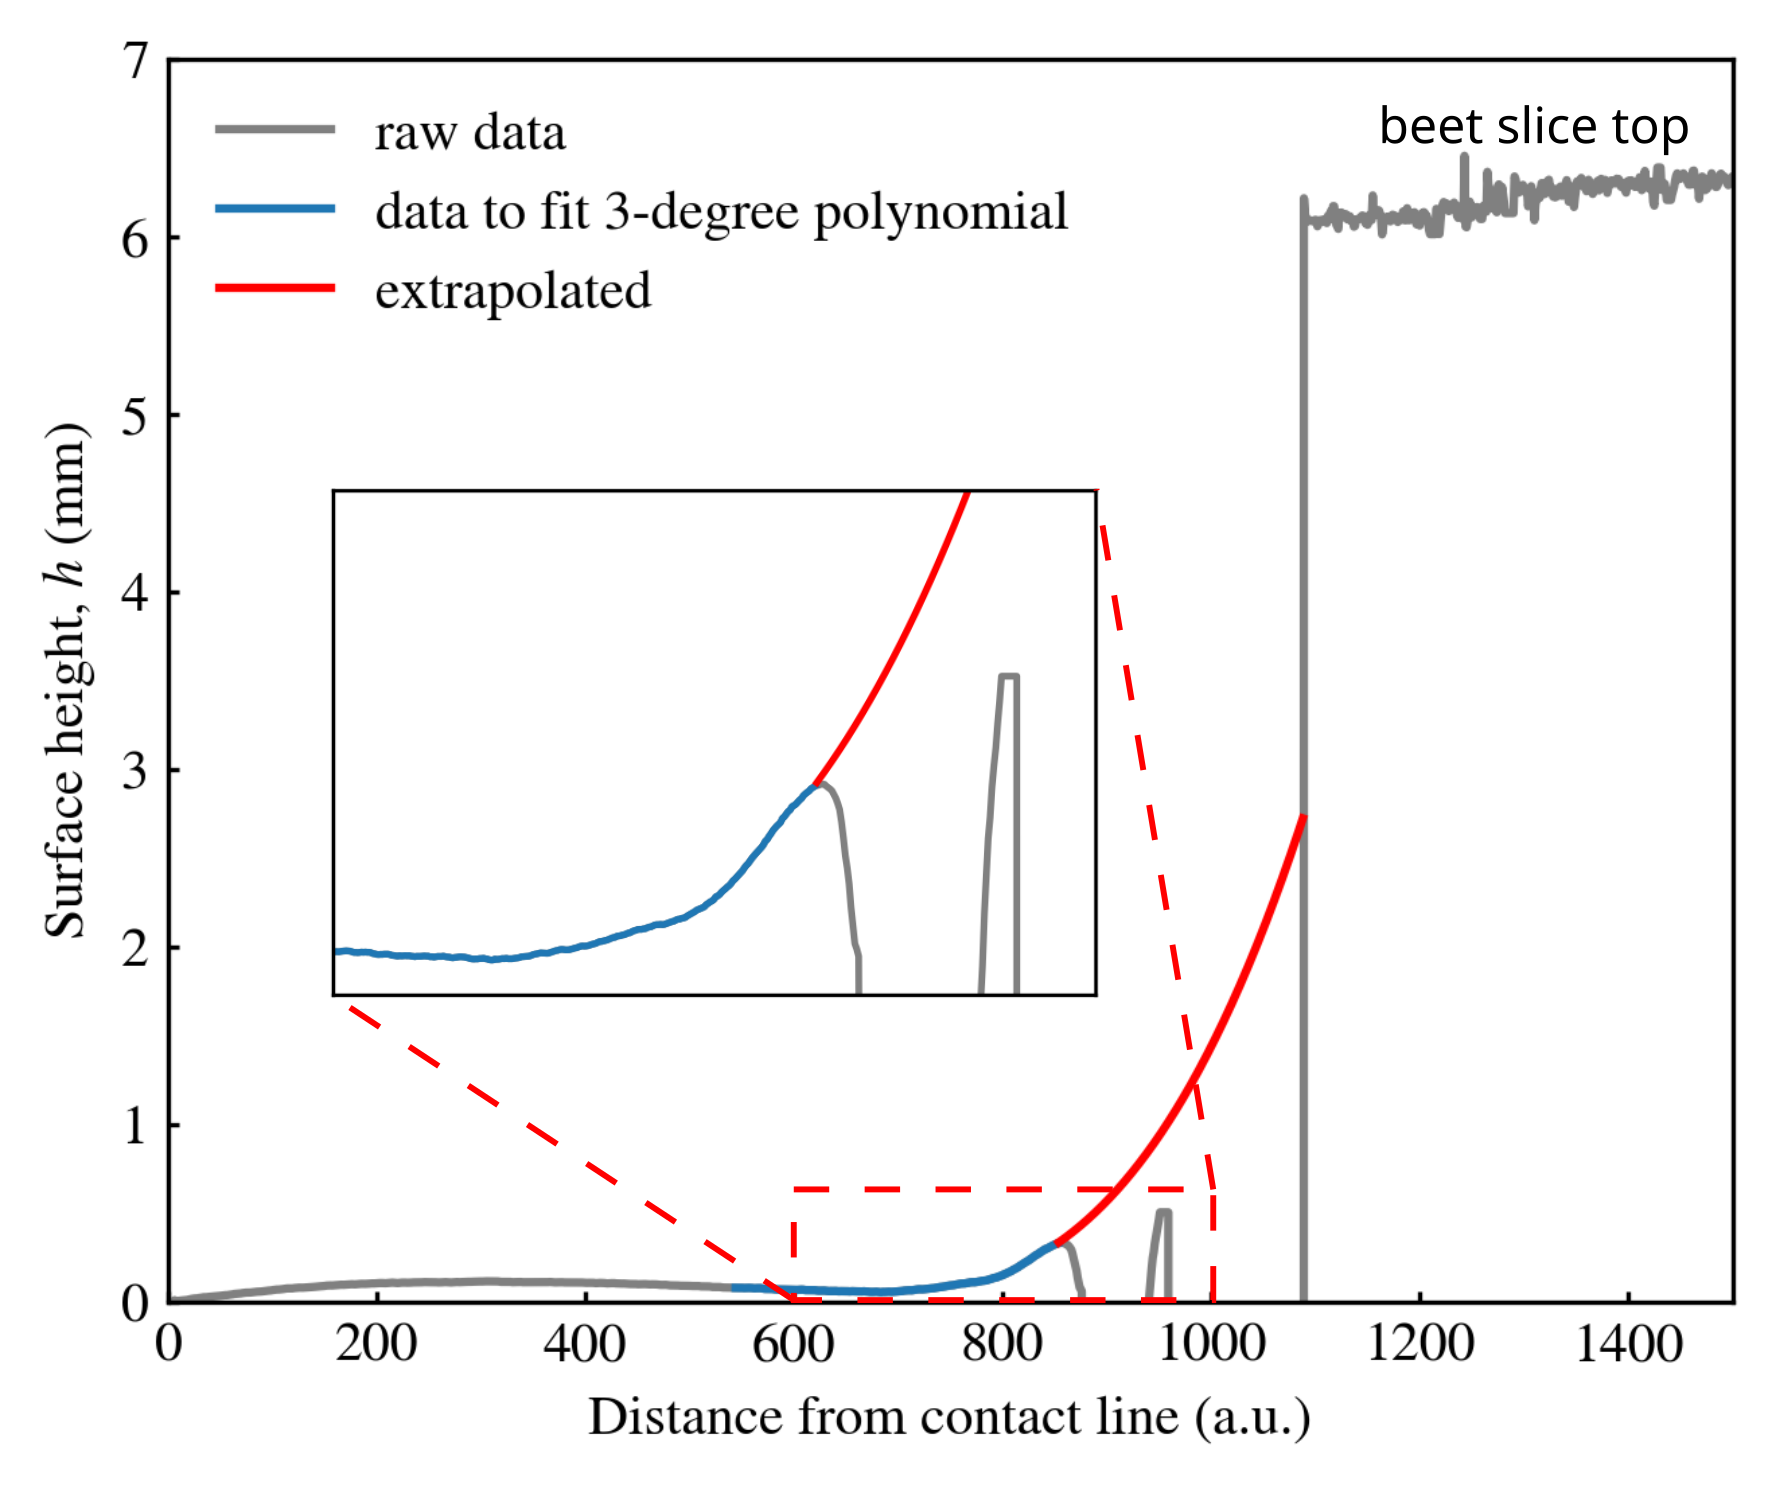
\includegraphics[width=\textwidth]{Figures/extrapolation_illustration.png}
    \caption{
    Illustration of the extrapolation method. 
    }
    \label{fig:extrapolation}
\end{figure}

\newpage

\section{Contact line dynamics measurements}

We measured the contact line dynamics by tracking the motion of the contact line, as well as the instantaneous contact angle. 
The coupling parameter $\kappa$ is then obtained by fitting the data with the Hoffman-de Gennes model. 
The results for the beet juice, 60\% glycerol and 80\% glycerol are shown in Table.~\ref{tab:contact-line-dynamics}.

\begin{table}[ht]
    \centering
    \begin{tabular}{cccc}
    \hline
    Liquid          & $\kappa\times 10^{4}$ & $\theta_s$ ($^\circ$) \\
    \hline
    Beet juice      & $2.2\pm 0.2$            & $17.4\pm 6.3$           \\
    60wt\% glycerol & $1.9\pm 1.3$            & $31.2\pm 0.3$          \\
    80wt\% glycerol & $5.2\pm 1.7$            & $32.5\pm 2.6$           \\
    \hline
    \end{tabular}
    \caption{
    Contact line velocity coupling factor $\kappa$ and static contact angle $\theta_s$.
    }
    \label{tab:contact-line-dynamics}
\end{table}

\newpage

\section{Influence of all the parameters}

Here, we simulate the surface profile evolutions varying all the parameters to assess their influence. The results are shown in Fig.~\ref{fig:all-parameters-influence}.

\begin{figure}[ht]
    \centering
    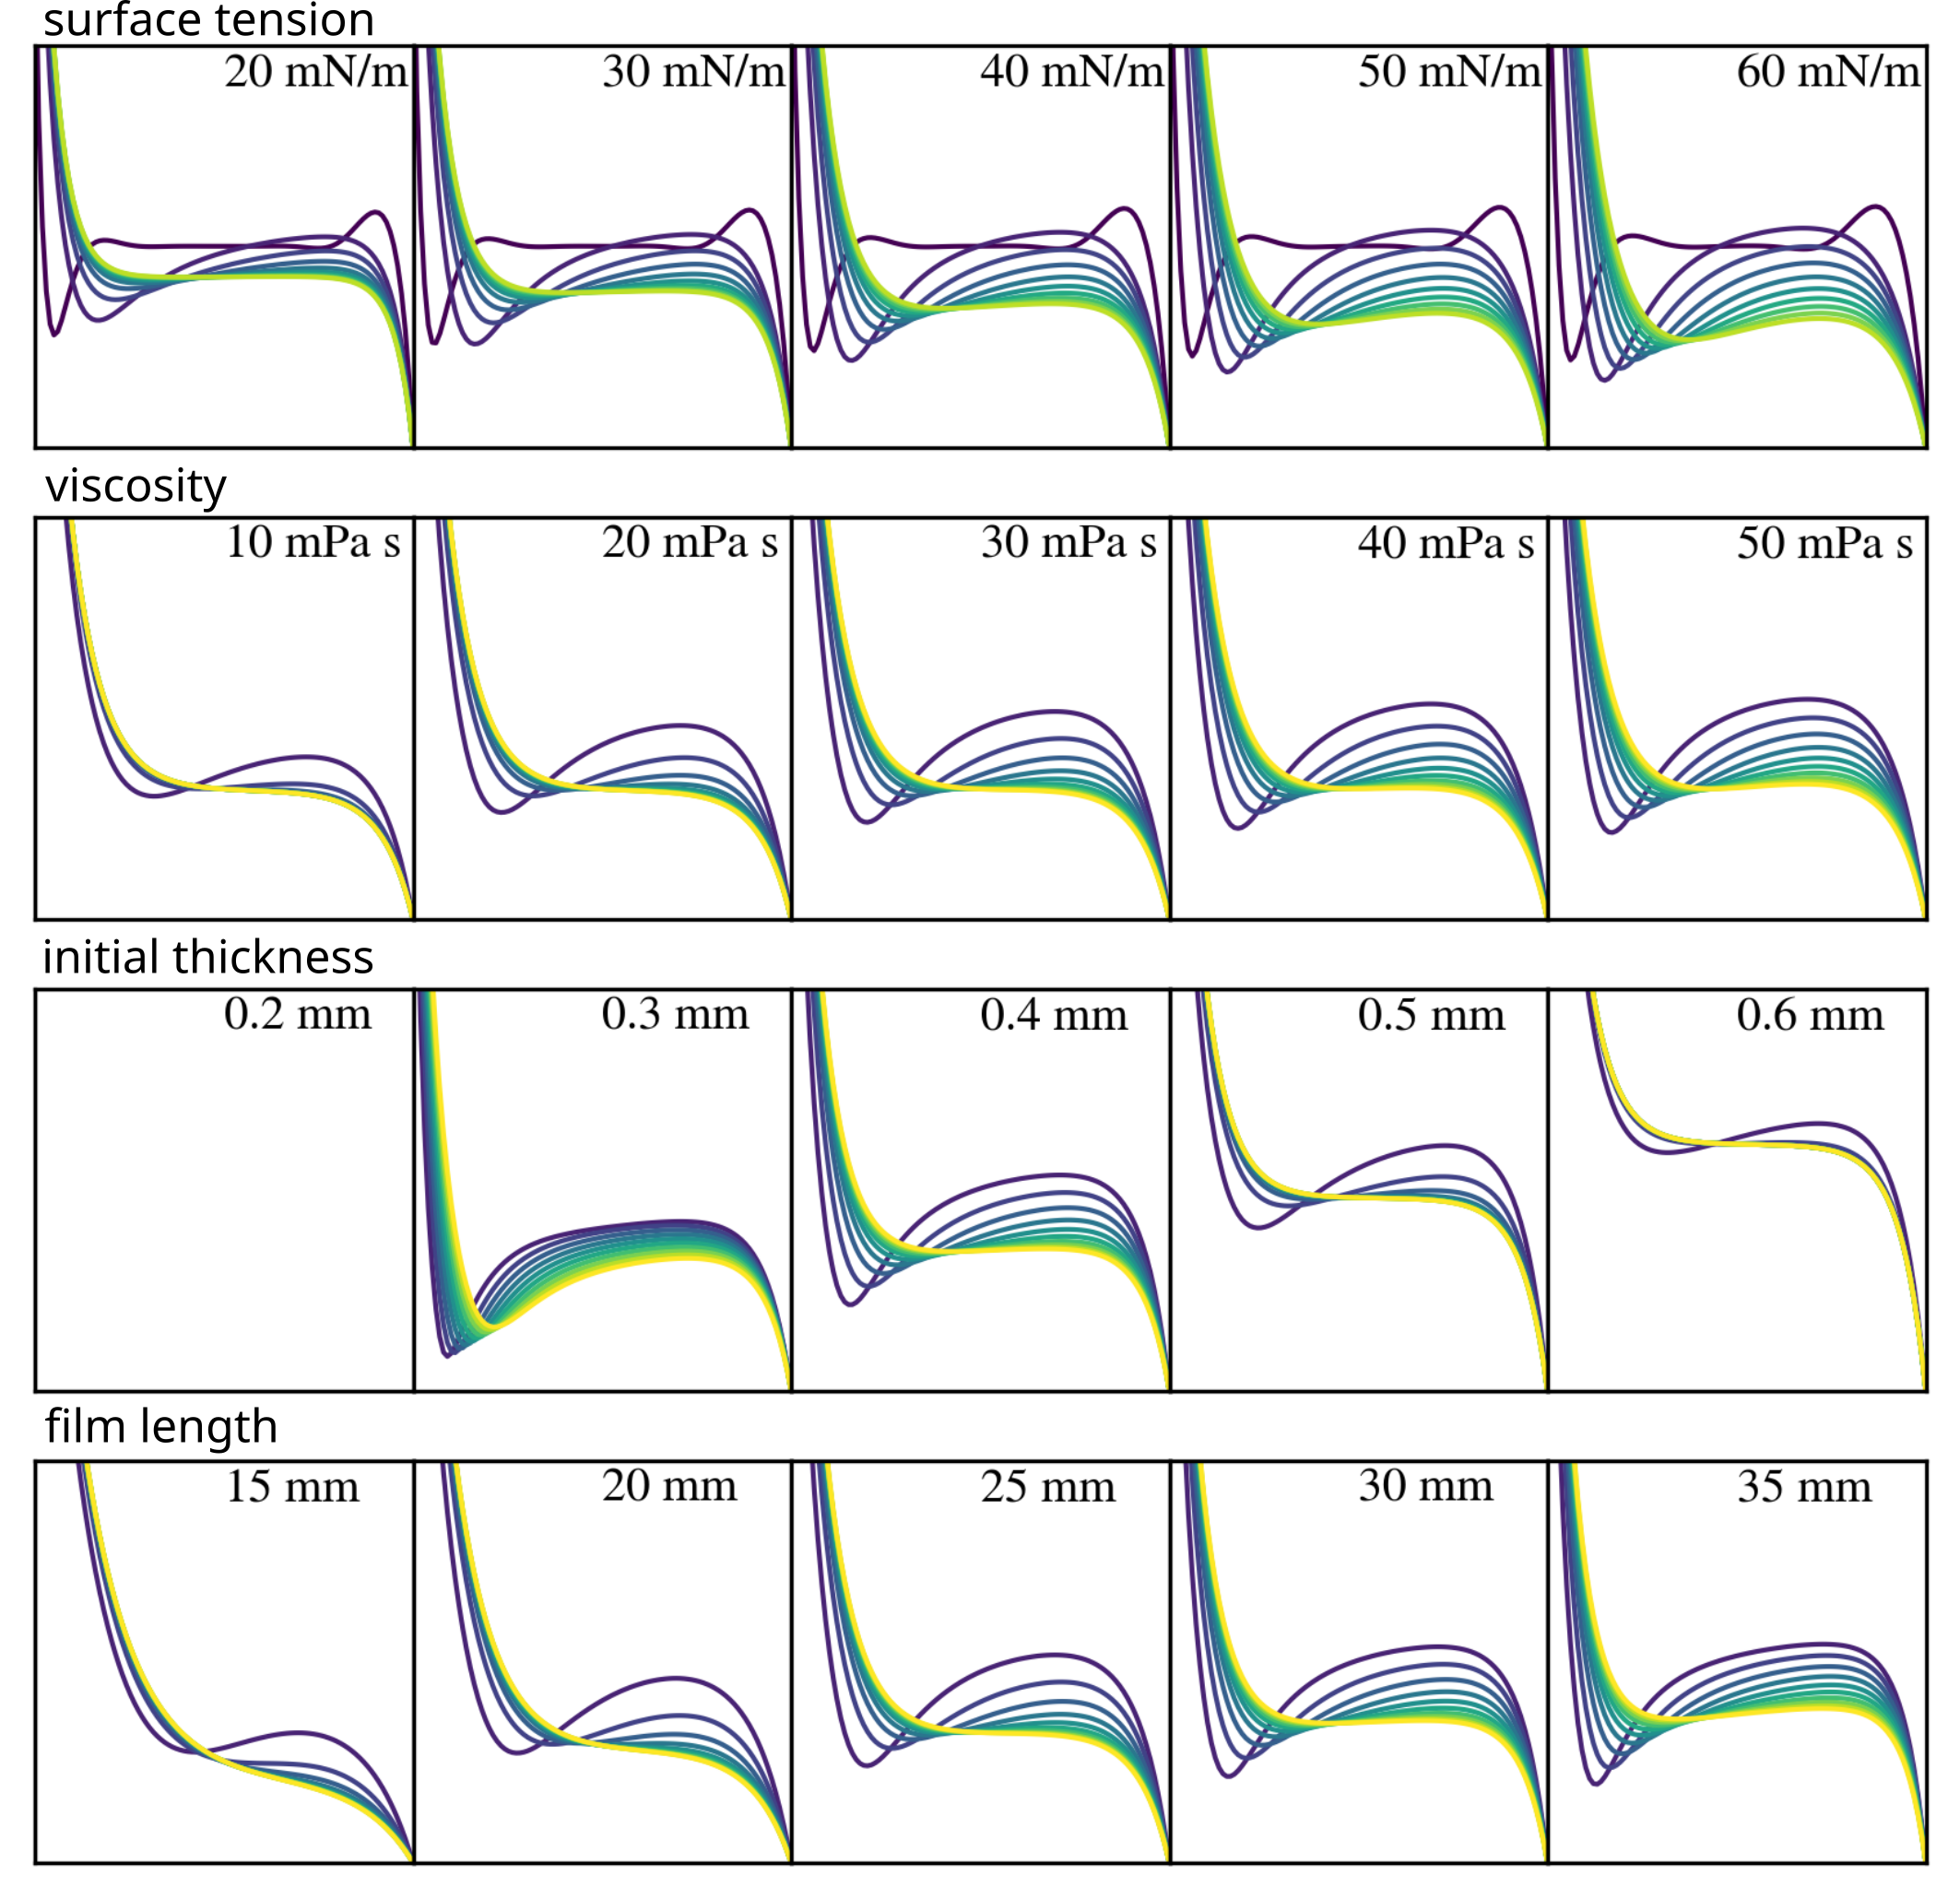
\includegraphics[width=\linewidth]{Figures/all_parameter_effects.png}
    \caption{
    Surface profile evolutions for various parameters.
    }
    \label{fig:all-parameters-influence}
\end{figure}

\newpage

\section{Relation between dimple thickness and initial thickness}

The dimple thickness $h$ and the initial film thickness $h_0$ are closely correlated. 
Generally, smaller $h_0$ leads to smaller dimple thickness. 
This relation is almost linear for large $h_0$, but can get highly non-linear for small $h_0$, as evidenced by the data shown in Fig.~\ref{fig:dimple-thickness-relation}.

\begin{figure}[ht]
    \centering
    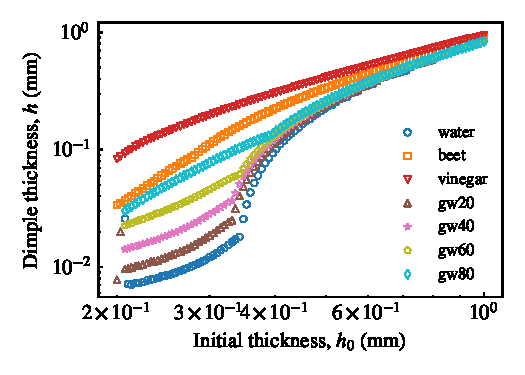
\includegraphics[width=\linewidth]{Figures/dimple_thickness}
    \caption{
    Dimple height at quasi-steady state plotted as a function of initial thickness $h_0$ from simulation, for various liquids. 
    }
    \label{fig:dimple-thickness-relation}
\end{figure}

\newpage

\section{Counterintuitive surface tension effect}

Although my scaling analysis predicts that the dimple time should decrease when surface tension gets large, the simulation results show that the dimple time actually increases. Detailed analysis shows that a fluid with higher surface tension reaches a lower height ratio at the beginning compared to a fluid with lower surface tension. This makes the dimple survive longer.

\begin{figure}[ht]
    \centering
    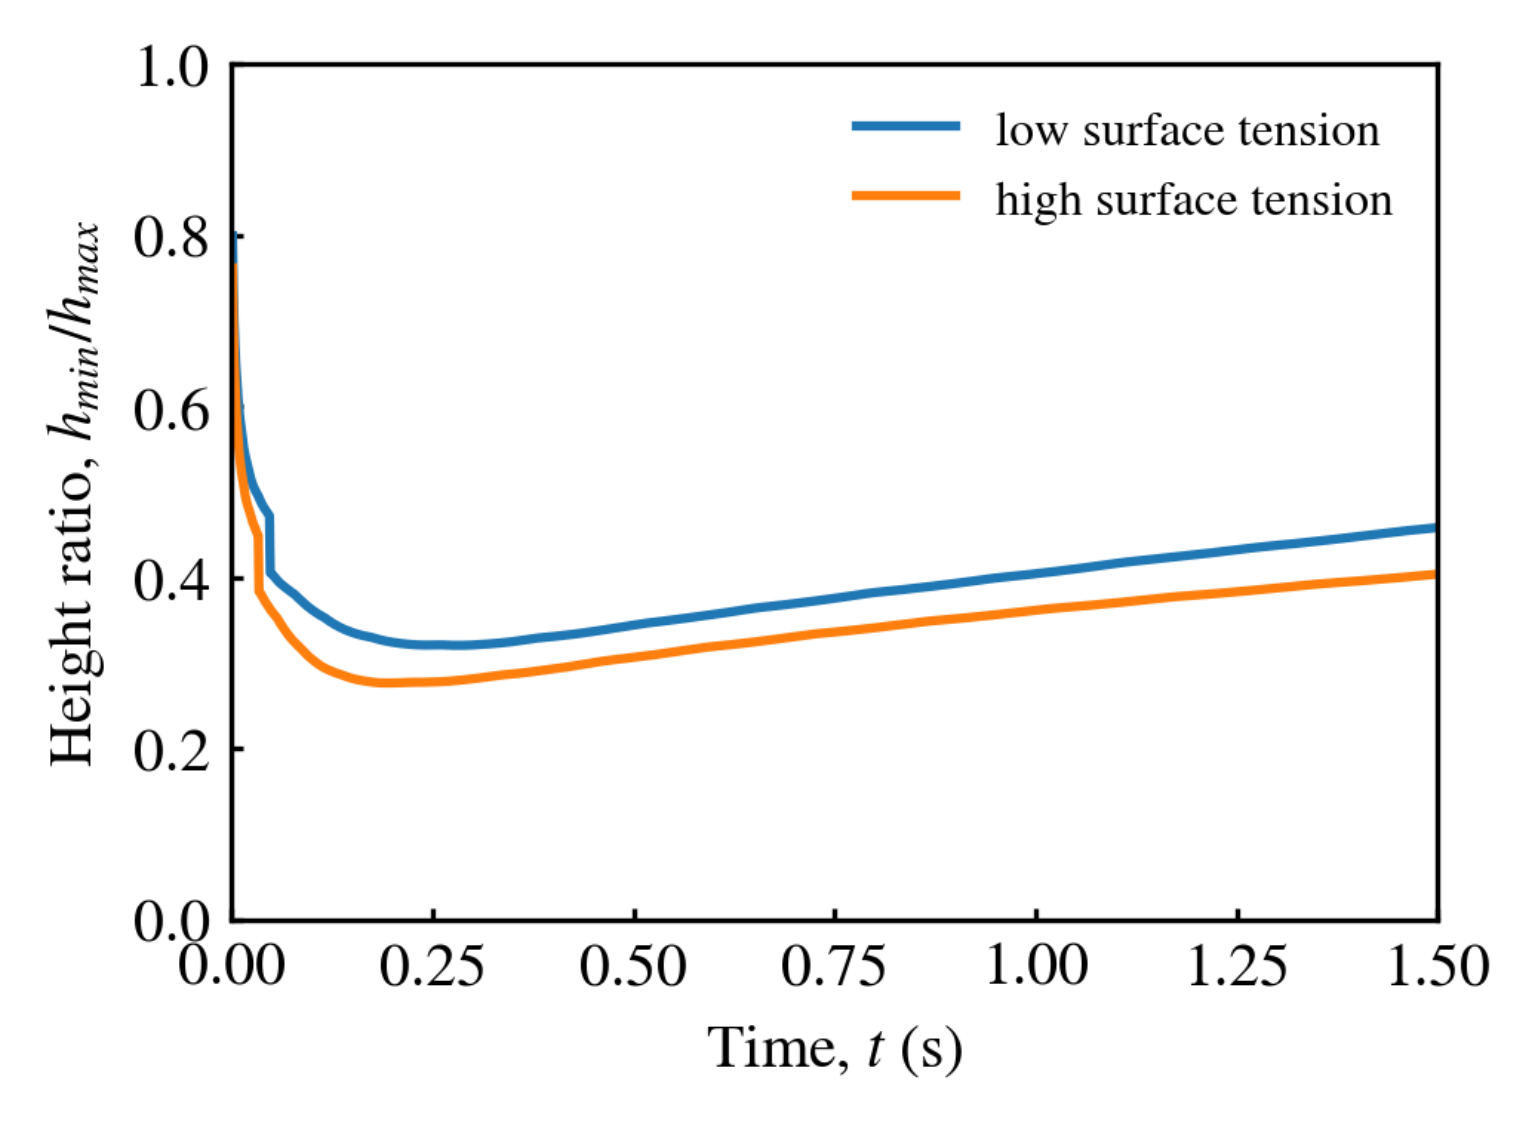
\includegraphics[width=\linewidth]{Figures/surface_tension_effect.png}
    \caption{
    Height ratio as a function of time for two liquids with different surface tensions. This is a simulation result.
    }
    \label{fig:surface-tension-effect}
\end{figure}

\newpage

\section{Dimple time data}

\begin{figure}[ht]
    \centering
    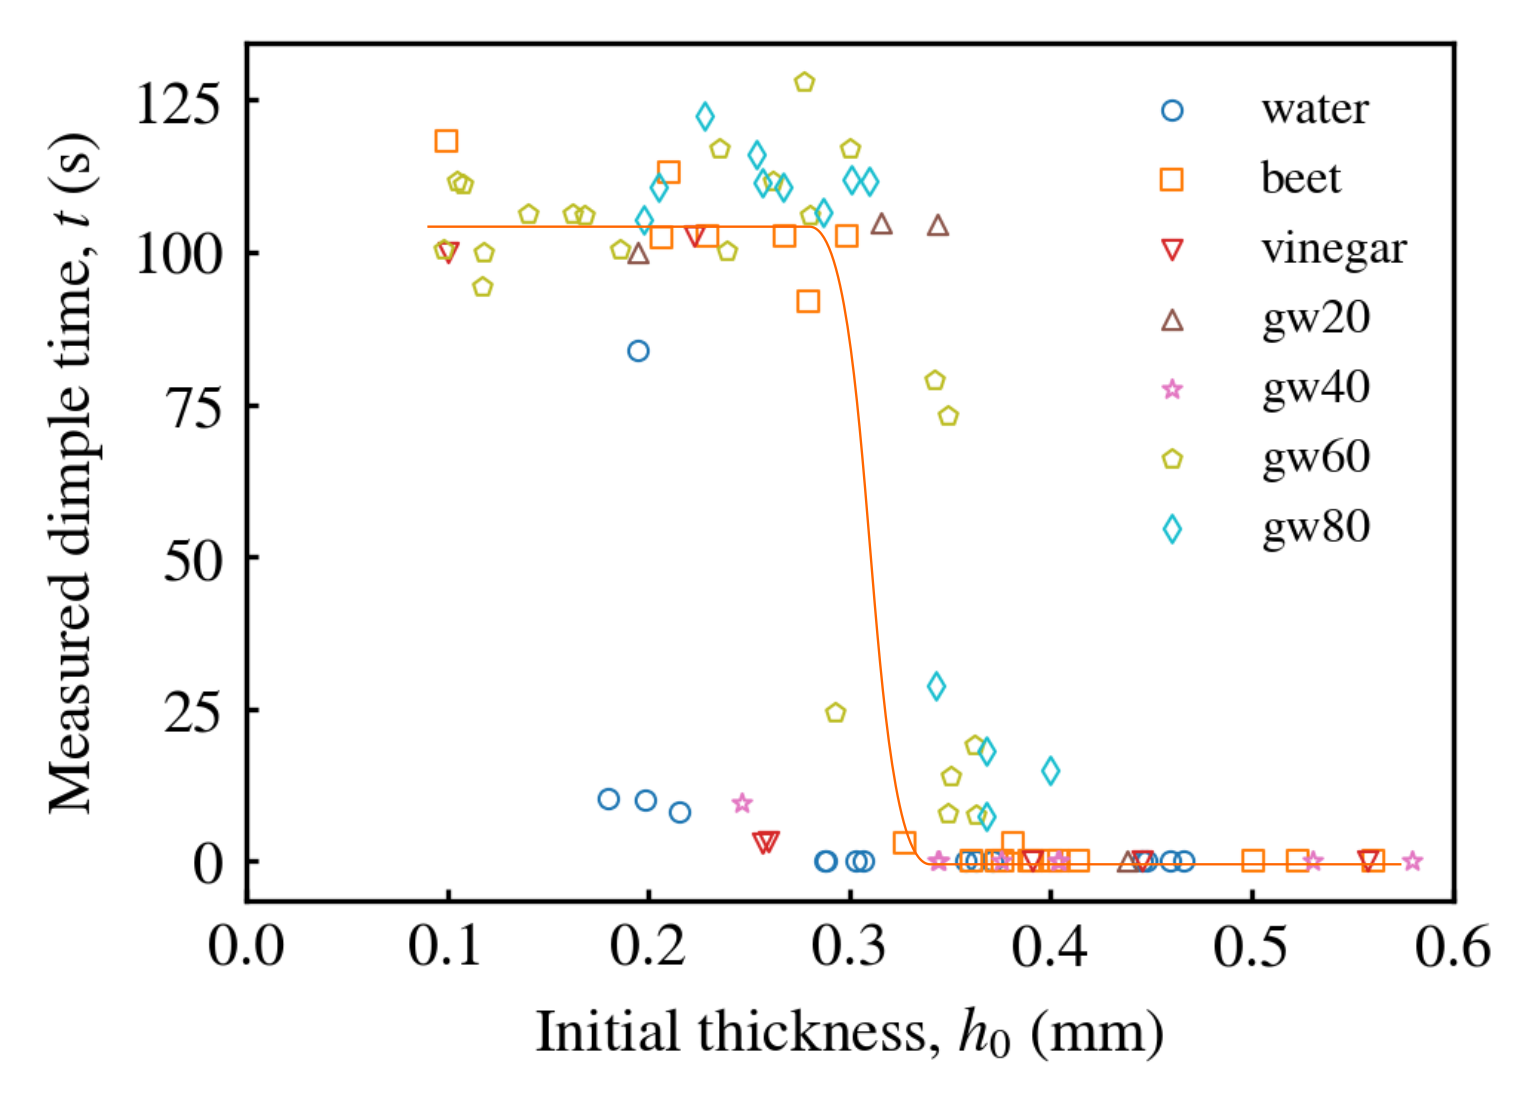
\includegraphics[width=\linewidth]{Figures/all_dimple_time_data}
    \caption{
    Alternative way to look at the dimple time data. Most of the times are either 0 or above 100 s, but a clear separation in the initial thickness $h_0$ can be identified, highlighting that long dimples are only observed for small $h_0$.
    }
    \label{fig:all-dimple-time-data}
\end{figure}

% \begin{thebibliography}{99}
% \bibitem{ref1} Author A. B., Author C. D., Journal Name \textbf{Volume}, Page (Year).
% \bibitem{ref2} Author E. F., Journal Name \textbf{Volume}, Page (Year).
% \end{thebibliography}

\newpage
\section{Supplementary Videos}

Video S1: Formation of the fringe around a beet slice.

Video S2: Bottom view of the scanning process (top), and the surface profiles measured by the displacement sensor (bottom). The video is played at real time. 

\end{document}
